\documentclass[a4paper, 10pt]{article}
\usepackage{header}




\title{\LARGE{Microeconomics-2 (advanced course)}\\
FES HSE}
\author{Viner Daniil  \href{https://t.me/danya_vin}{@danya\_vin}}
\date{Last update \today}

\begin{document}
\maketitle
\tableofcontents
\newpage
\setlength{\parindent}{15pt}
\setlength{\parskip}{2mm}
\section{Classic monopoly}
\subsection{Definition}
A firm is \textbf{a monopoly} if no other firms produces the same good or a close substitute.

\comment We differentiate among the products referring to the cross-price elasticity: if its value is small, then the potential substitutes are not close enough to be a substitute.

A monopolist has market power in the sense that the amount of output that it is able to sell responds continuously on the price it charges.

Obviously, that the monopolist suggests consumers a good at a price of $p$. 

\subsection{Examples of a monopoly}
The main reason why a monopoly exists is the fact that other firms find it impossible or unprofitable to enter the market (or to continue the competition with more bigger firms).

The greatest examples of a monopoly are:
\begin{itemize}
    \item Natural monopolies, when a single company can produce and offer to sell a product or service at a lower cost than its competitors can
    \item Legal protection of a patent holder, when the government prohibits using some technologies, ideas and producing methods except by those who created them
\end{itemize}


\subsection{Model of a monopoly}
Let’s suppose there are many consumers of a good and they are price-takers. We'll assume that a good which we're considering is normal, which means that the function of demand — $D(p)$ is decreasing.

$y=D(p)$ — the output if the monopoly, $c(y)$ — costs function of the firm-monopolist.

So, the monopolist chooses the price $p^m$ which is the solution of the maximization problem:
\begin{equation}\label{eq:1.3.1}
    \Pi(p)=pD(s)-c(D(p))\longrightarrow\max_{p\geqslant0}
\end{equation}

Logically, $y^m=D(p^m)$ is the output of the monopolist.

Sometimes it's easier to use an inverse function $p=p(y)=D^{-1}(y)$.

Then, output $y^m$ is the solution of this problem:
\begin{equation}\label{eq:1.3.2}
    \Pi(y)=p(y)y-c(y)\longrightarrow\max_{y\geqslant0}
\end{equation}

\subsection{First-order condition}
\begin{equation}
    \begin{cases}
        \Pi'(y^m)\leqslant 0\\
        y^m\cdot\Pi(y^m)=0
    \end{cases}
\end{equation}
\indent Condition that $y^m>0$ is guaranteed by:
\begin{equation}
    p(0)>c'(0)
\end{equation}

\textbf{Proof.} If $y^m=0$, next condition must be done:
\begin{equation*}
    \Pi'(0)=p(0)-c'(0)\leqslant 0
\end{equation*}
which contradicts $p(0)>c'(0)$\qed

\begin{equation}
    \begin{aligned}
        \Pi(y)&=p(y)y-c(y)\\
        \Pi'(y)&=\left(p(y)y-c(y)\right)^{\prime}=0\\
        &=p(y)\cdot p'(y)y=c'(y),\quad \text{at }y=y^m>0
    \end{aligned}
\end{equation}

Then, $p^m=p(y^m)$

Let's $TC=D(p)p$, $TC=c(D(p))$, then as we maximize $\Pi$
\begin{equation*}
    \begin{aligned}
        \Pi'&=0\\
        TR'-TC'&=0\\
        MR-MC&=0
    \end{aligned}
\end{equation*}

$$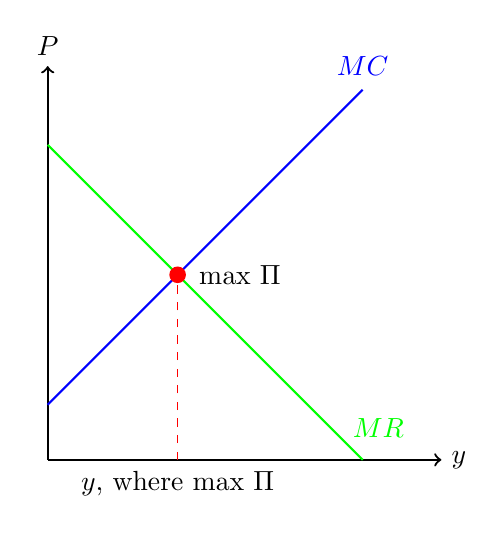
\begin{tikzpicture}[scale=2]

    \draw[thick,->] (0,0) -- (2.5,0) node[right] {$y$}; 
    \draw[thick,->] (0,0) -- (0,2.5) node[above] {$P$}; 

    \draw[thick, green] (0,2) -- (2,0);
    \draw[thick, blue] (0,0.35) -- (2,2.35);
    
    \fill[red] (0.825,1.175) circle (1.5pt);
    \node[anchor=west, black] at (0.9,1.175) {max $\Pi$};

    \draw[dashed, red] (0.825,0) -- (0.825,1.175);

    \node[black] at (0.825,-0.15) {$y$, where max $\Pi$};
    \node[blue] at (2,2.5) {$MC$};
    \node[green] at (2.1,0.2) {$MR$};

\end{tikzpicture}$$
\subsection{Second-order condition}
Let $TR(y)=p(y)y$ and $MR(y)=TR'(y)$, then
\begin{equation}
    \left(MR(y^m)\right)'<\left(MC(y^m)\right)'
\end{equation}
\subsection{Illustration of the monopolist problem}
$$
\begin{tikzpicture}[scale=2]

    \draw[thick,->] (0,0) -- (4,0) node[right] {$y$}; 
    \draw[thick,->] (0,0) -- (0,4) node[above] {$P$};

    \draw[thick, blue] (0,3.5) -- (1.9,0); %MC
    \draw[thick, green] (0.5,1) .. controls (2,1) and (2,2.2) .. (2.05,2.2); %MR 
    \draw[thick, red] (0,3.5) -- (3.8,0);

    \fill[teal] (1.28,2.33) circle (1.5pt);


    \draw[dashed, teal] (1.28,0) -- (1.28,2.33);
    \draw[dashed, teal] (0,2.33) -- (1.28,2.33);
    \node[anchor=east, teal] at (0,2.33) {$p^m$};
    \node[anchor=north east, teal] at (1.38,0) {$y^m$};
    \node[anchor=north west, blue] at (1.9,0.3) {$MR$};
    \node[anchor=north west, red] at (3.6,0.5) {$p(y)=D^{-1}(y)$};
    \node[green] at (2.2,2.1) {$MC$};
    
\end{tikzpicture}
$$

Here $p^m$ and $y^m$ are the price and output at which customers will buy the volume of good at which $MR=MC$.

\subsection{Inverse elasticity pricing rule}
\definition 
\begin{equation}\label{eq:1.7.1}
    \frac{p^m-MC(y^m)}{p^m}=\frac{1}{|\varepsilon_d|},\quad \text{for }|\varepsilon_d|>1
\end{equation}

The right part of the formula (\ref{eq:1.7.1}) is called \textbf{Lerner's Index}. It shows the degree of the monopoly power. At the same time it shows how the mark-up price depends on the elasticity of demand. 

\comment If the elasticity of demand is infinite, then the firm is a price taker and has no market power.

\comment The greater the elasticity, the smaller the markup the manufacturer can make because in that case customers will refuse to consume.

Let's find the formula (\ref{eq:1.7.1}) by mathematical transformation. We know that:
\begin{itemize}
    \item $p'(y^m)y^m+p(y^m)=c'(y^m)$
    \item $p(y^m)=c'(y^m)$
    \item $\varepsilon_d=\displaystyle\frac{\text{d}y}{\text{d} p}\cdot\frac{p}{y}<0$
\end{itemize}
So, transform by using that equations we get
$$\begin{aligned}
    p(y^m)\left[1+\displaystyle\frac{p'(y^m)y^m}{p(y^m)}\right]&=c'(y^m)\\
    p^m\left[1-\displaystyle\frac{1}{|\varepsilon_d|}\right]&=c'(y^m)\\
    p^m-\displaystyle\frac{p^m}{|\varepsilon_d|}&=c'(y^m)\\
    \displaystyle\frac{p^m-c'(y^m)}{p^m}&=\frac{1}{|\varepsilon_d|}\\
    \frac{p^m-MC(y^m)}{p^m}&=\frac{1}{|\varepsilon_d|}
\end{aligned}$$

\subsection{Monopoly's output in comparison with the perfectly competitive industry}
Consider a monopoly with the $c(y) \in C^1$ costs function and a perfectly competitive industry with the same costs $c(y)$.Let $p(y) \in C^1$ be an inverse demand function. Then given $p' > 0,\ c' > 0,\ c'' > 0$ and $p(0) > c'(0)$

\noindent
\begin{minipage}{0.5\textwidth}
\proposition The monopoly output $y^m$ will be less than the output $\overline{y}$ of the perfectly competitive industry
\begin{equation}\label{eq:1.8.1}
    y^m<\overline{y}
\end{equation}

\proof It's simple. On the one hand, $y^m$ maximizes $\Pi$ of the monopoly, then
$$p(y^m)y^m-c(y^m)\geqslant p(\overline{y})\overline{y}-c(\overline{y})$$

On the other hand, $\overline{y}$ provides maximum profit to the price-taking firm at a constant price $p(\overline{y})$, then
$$p(\ov{y})\ov{y}-c(\ov{y})\geqslant p(\ov{y})y^m-c(y^m)$$

Adding these equations we get $p(y^m)y^m\geqslant p(\ov{y})y^m\Longrightarrow\boxed{y^m<\ov{y}}$\footnote{Remember, that $p(y)$ is an inverse function of demand and $y^m\ne \ov{y}$ because of $p(\ov{y})-c'(\ov{y})\leqslant0$}
\end{minipage}
\begin{minipage}{0.5\textwidth}
$$
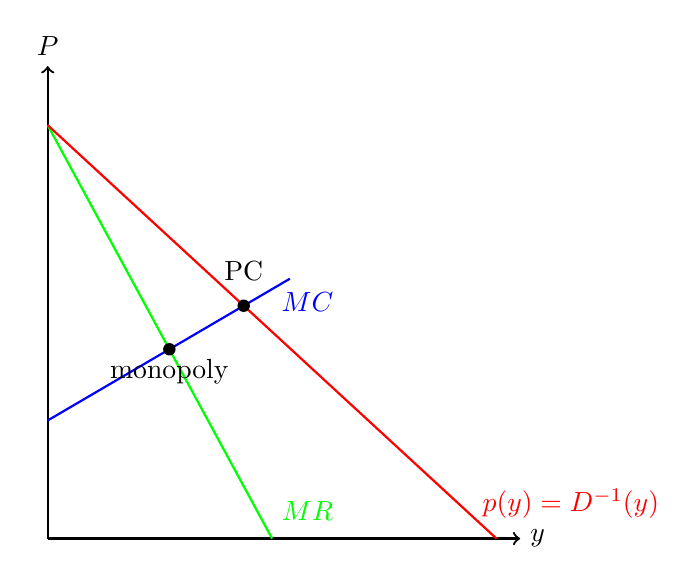
\begin{tikzpicture}[scale=1.5]

    \draw[thick,->] (0,0) -- (4,0) node[right] {$y$}; 
    \draw[thick,->] (0,0) -- (0,4) node[above] {$P$};

    \draw[thick, green] (0,3.5) -- (1.9,0); 
    \draw[thick, blue] (0,1) -- (2.05,2.2); 
    \draw[thick, red] (0,3.5) -- (3.8,0); %p(y)

    \fill[teal, black] (1.02988, 1.60286) circle (1.5pt);
    \fill[teal, black] (1.65957, 1.97145) circle (1.5pt);

    \node[anchor=north west, green] at (1.9,0.4) {$MR$};
    \node[anchor=north west, red] at (3.6,0.5) {$p(y)=D^{-1}(y)$};
    \node[blue] at (2.2,2) {$MC$};
    \node[anchor=south, black] at (1.65957, 2.1) {\text{PC}};
    \node[anchor=north, black] at (1.02988, 1.60286) {\text{monopoly}};
    
\end{tikzpicture}
$$
\end{minipage}
\subsection{Comparative Statics}
Let $p(y)\in C^2,\ p' <0,\ MC =c,\ p(0)>c,\ (MR)' <0$. Then
\begin{equation*}
    \frac{dy^m(c)}{dc}<0\quad \text{and}\quad\frac{dp^m(c)}{dc}>0
\end{equation*}

\section{Quasilinear Economy}
Consider an economy where there are $m$ consumers and $n$ firms. All of consumers have quasilinear preferences, for $i$-th consumer his utility is $U_i(x_i,z_i)=v_i(x_i)+z_i$, where $x_i$ is the only good to be consumed and $z_i$ is the money owned by this consumer.

Properties of $v_i(x_i)$ functions:
\begin{itemize}
    \item $v_i'(x_i)>0$
    \item $v_i''(x_i)<0$
    \item $v_i(0)=0$
\end{itemize}

\subsection{Main theorem of the quasilinear economy}
Let $\bar{x}=\left(x_1, x_2, \ldots, x_m\right), \bar{y}=\left(y_1, y_2, \ldots, y_n\right), \bar{r}=\left(r_1, r_2, \ldots, r_n\right)$ and $\bar{z}=\left(z_1, z_2, \ldots, z_m\right)$

Allocation $(\widehat{\bar{x}}, \widehat{\bar{y}}, \widehat{\hat{r}}, \widehat{\bar{z}})$ is Pareto-optimal if and only if it is a solution of the problem
\begin{equation}\label{eq:2.1.1}
\left\{\begin{array}{l}
\sum_i \nu_i\left(x_i\right)-\sum_j c_j\left(y_j\right) \longrightarrow \max \\
\sum_i\left(x_i\right) \leq \sum_i y_j \\
x_i \geq 0,\ y_j \geq 0 \\
\text {for all } i \in I \text { and } j \in J
\end{array}\right.
\end{equation}


Moreover $\widehat{r_j}=c_j\left(\widehat{y_j}\right)$ and $\sum_i \widehat{z_i}=\sum_i w_i-\sum_j \widehat{r_j}$.

\subsection{Welfare analysis under monopoly}
The first line in (\ref{eq:2.1.1}) is the main goal of consumers, i.e. to maximize the welfare. That function is called a \textbf{welfare indicator}. Then we have $2$ sets of indices, $I = \{1,2,\ldots,m\}$ and
$J = \{1,2,\ldots,n\}$.

At \textit{Pareto-optimal allocation} it takes the maximum value $W_{max}$. If an allocation \textit{is not} Pareto-optimal, then $W < W_{max}$ and this difference $W_{max} - W$ is called \textbf{deadweight loss} $(DWL)$.

We give the following definitions for Consumers’ ($CS$) and producers’ ($PS$) surplus:
\begin{equation}
    \begin{aligned}
        CS&=&\sum_{i\in I}\nu_i(x_i)-p\sum_{i\in I}x_i\\
        PS&=&p\sum_{j\in J}y_j-\sum_{j\in J}c_j(y_j)
    \end{aligned}
\end{equation}

Welfare indicator at $(x, y)$ allocation equals $W (x, y) = CS + PS$. Moreover, we can identify $$W=\sum_{i=1}^m v_i(x_i)-c(y)$$

Let $y=\sum_{i\in I}x_i=x$ — output of a monopoly

\begin{enumerate}
    \item $W(y)=v(y)-c(y)\longrightarrow\max\limits_{y>0}\Longrightarrow v'(y)=c'(y)$
    \item First-order condition:
    \begin{equation*}
        \begin{aligned}
            \left(p(y)y\right)'-c'(y)&=0\\
            p'(y)y+p(y)-c'(y)&=0
        \end{aligned}
    \end{equation*}
    \item If we differentiate the formula $W(y)=v(y)-c(y)$:
    \begin{equation*}
        \begin{aligned}
            W'(y^m)&=v'(y^m)-c'(y^m)>0\\
            &=p(y^m)-c'(y^m)\\
            &=-p'(y^m)y^m>0
        \end{aligned}
    \end{equation*}
\end{enumerate}

$$
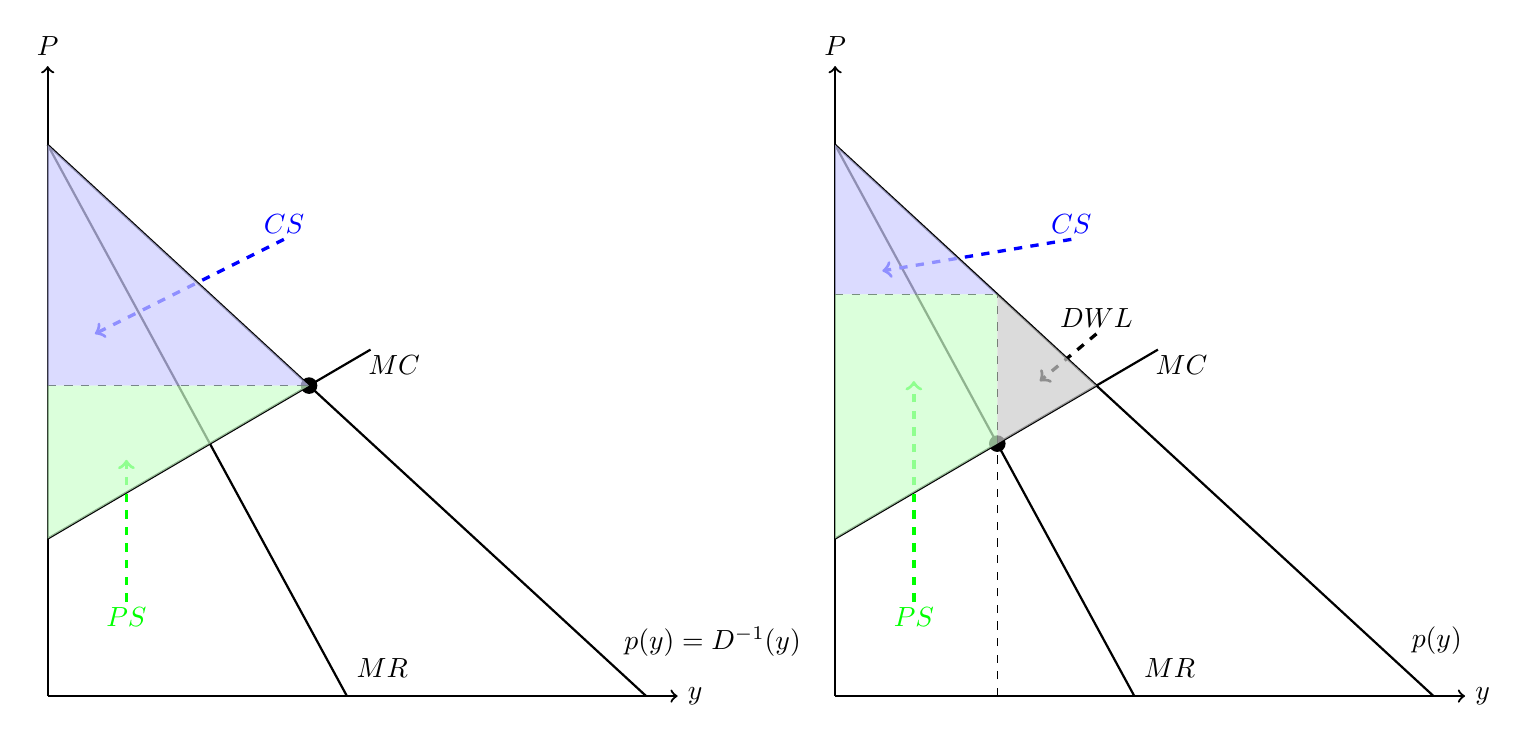
\begin{tikzpicture}[scale=2]

    \draw[thick,->] (0,0) -- (4,0) node[right] {$y$}; 
    \draw[thick,->] (0,0) -- (0,4) node[above] {$P$};

    \draw[thick, black] (0,3.5) -- (1.9,0); 
    \draw[thick, black] (0,1) -- (2.05,2.2); 
    \draw[thick, black] (0,3.5) -- (3.8,0);
    \draw[very thick, dashed, blue, ->] (1.5,2.9) -- (0.3,2.3);
    \draw[very thick, dashed, green, ->] (0.5,0.6) -- (0.5,1.5);
    \draw[dashed] (0,1.97145) -- (1.65957, 1.97145);

    \fill[teal, black] (1.65957, 1.97145) circle (1.5pt);

    \node[anchor=north west, black] at (1.9,0.3) {$MR$};
    \node[anchor=north west, black] at (3.6,0.5) {$p(y)=D^{-1}(y)$};
    \node[black] at (2.2,2.1) {$MC$};
    \node[blue] at (1.5,3) {$CS$};
    \node[green] at (0.5,0.5) {$PS$};
    \fill[fill=blue!20,opacity=0.7] 
        (0, 1.97145) -- (1.65957, 1.97145) -- (0,3.5) -- cycle;

    \fill[fill=green!20,opacity=0.7] 
        (0, 1) -- (1.65957, 1.97145) -- (0, 1.97145) -- cycle;

    \begin{scope}[shift={(5,0)}]
        \draw[thick,->] (0,0) -- (4,0) node[right] {$y$}; 
        \draw[thick,->] (0,0) -- (0,4) node[above] {$P$};

        \draw[thick, black] (0,3.5) -- (1.9,0); 
        \draw[thick, black] (0,1) -- (2.05,2.2); 
        \draw[thick, black] (0,3.5) -- (3.8,0);
        \draw[very thick, dashed, blue, ->] (1.5,2.9) -- (0.3,2.7);
        \draw[very thick, dashed, green, ->] (0.5,0.6) -- (0.5,2);
        \draw[dashed] (1.02988, 0) -- (1.02988, 2.55);
        \draw[dashed] (0,2.55) -- (1.02988, 2.55);
        \draw[very thick, dashed, ->] (1.65957, 2.3) -- (1.3, 2);

        \node[anchor=north west, black] at (1.9,0.3) {$MR$};
        \node[anchor=north west, black] at (3.6,0.5) {$p(y)$};
        \node[black] at (2.2,2.1) {$MC$};
        \node[blue] at (1.5,3) {$CS$};
        \node[green] at (0.5,0.5) {$PS$};
        \node[black] at (1.65957, 2.4) {$DWL$};
        \fill[teal, black] (1.02988, 1.60286) circle (1.5pt);
        

        \fill[fill=blue!20,opacity=0.7] 
            (0, 2.55) -- (1.02988, 2.55) -- (0,3.5) -- cycle;

        \fill[fill=green!20,opacity=0.7] 
            (0, 1) --(0, 2.55)-- (1.02988, 2.55) --(1.02988, 1.60286)-- cycle;

        \fill[fill=black!20,opacity=0.7] 
            (1.02988, 1.60286) --(1.02988, 2.55)-- (1.65957, 1.97145) -- cycle;
        
    \end{scope}
    
\end{tikzpicture}
$$

\subsection{DWL formula}
\noindent
\begin{minipage}{0.5\textwidth}
    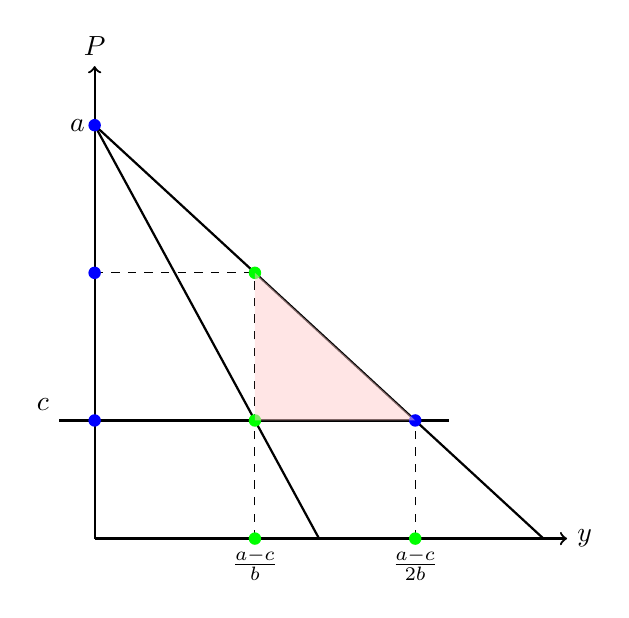
\begin{tikzpicture}[scale=1.5]
        \draw[thick,->] (0,0) -- (4,0) node[right] {$y$}; 
        \draw[thick,->] (0,0) -- (0,4) node[above] {$P$};
    
        \draw[thick, black] (0,3.5) -- (1.9,0); 
        \draw[thick, black] (-0.3,1) node[above left] {$c$} -- (3,1); 
        \draw[thick, black] (0,3.5) -- (3.8,0); %p(y)
        \draw[dashed] (1.35722, 0) -- (1.35722, 2.25);
        \draw[dashed] (0,2.25) -- (1.35722, 2.25);
        \draw[dashed] (2.71444, 0) -- (2.71444, 1);
    
        \fill[teal, green] (1.35722, 1) circle (1.5pt);
        \fill[teal, green] (1.35722, 2.25) circle (1.5pt);
        \fill[teal, blue] (2.71444, 1) circle (1.5pt);
        \fill[teal, blue] (0, 1) circle (1.5pt);
        \fill[teal, blue] (0, 3.5) circle (1.5pt) node[left, black] {$a$};
        \fill[teal, blue] (0,2.25) circle (1.5pt);
        \fill[teal, green] (1.35722, 0) circle (1.5pt) node[below, black] {$\frac{a-c}{b}$};
        \fill[teal, green] (2.71444, 0) circle (1.5pt) node[below, black] {$\frac{a-c}{2b}$};

        \fill[fill=red!20,opacity=0.5] 
            (1.35722, 1) --(1.35722, 2.25)-- (2.71444, 1) -- cycle;
    \end{tikzpicture}
\end{minipage}
\begin{minipage}{0.5\textwidth}
    For instance, we have $p(y)=a-by$ and $c'(y)=c$ then
    $$\begin{aligned}
        TR&=ay-by^2\\
        MR&=a-2by
    \end{aligned}$$

    Now, how try to find $DWL$? Optimal output will be $\hat{y}=\displaystyle\frac{a-c}{b}$, while monopoly's:
    $$y^m=\displaystyle\frac{a-c}{2b}$$
    So,
    $$DWL=\int_{y^m}^{\hat{y}}\left[(a-bt)-c\right]dt=\displaystyle\frac{(a-c)^2}{8b}$$
\end{minipage}%

\subsection{The concept of a representative consumer}
If an aggregate demand on good can be represented by solving a utility maximization problem of a sole consumer, then we say that in such economy a representative consumer exists. This is exactly the case in a quasilinear economy.

In other words there exists a function $\nu(x)$ such that by solving the problem
\begin{equation}
    \begin{cases}
        \nu(x)+\sum_{i \in I} z_i \rightarrow \max \\
        p \cdot \sum_{i \in I} x_i+\sum_{i \in I} z_i \leq \sum_{i \in I} w_i
    \end{cases}
\end{equation}
we can find the aggregate demand function $D(p) =\sum_{i\in I}x_i(p)$


\end{document}